% THIS TEMPLATE IS A WORK IN PROGRESS
% Adapted from an original template by faculty at Reykjavik University, Iceland

\documentclass{scrartcl}

% Adapted from an original template by Hlyni Arnórssyni, Reykjavik University, Iceland
%
% ------------------------------ SETTINGS
\usepackage{geometry}

\geometry{
	paper=a4paper, % Paper size
	top=2.5cm, % Top margin
	bottom=2.5cm, % Bottom margin
	left=2.5cm, % Left margin
	right=2.4cm, % Right margin
	headheight=0.75cm, % Header height
	footskip=1.5cm, % Space from the bottom margin to the baseline of the footer
	headsep=0.75cm, % Space from the top margin to the baseline of the header
	%showframe, % Uncomment to show how the type block is set on the page
}

\usepackage{blindtext}
%-------------------------------- Character encoding ----------------------------
\usepackage[T1]{fontenc}
\usepackage[utf8]{inputenc}

%----------------------------- Mathematics packages from AMS ---------------

\usepackage{amsmath, amsfonts, amsthm, amssymb}
\usepackage{braket, nicefrac}

% ----------- International System of Units
\usepackage{siunitx}

%------------------------------ Lists / numbers -------------------------
\usepackage{enumitem, multicol}

%------------------------------- Figure insertions --------------
\usepackage{graphicx, float}  % Use option [H] to force the placement of a figure
\usepackage{keystroke}
\usepackage{pgfplots}\usepgfplotslibrary{units}\pgfplotsset{compat=1.16}




%%%%%%%%%%%%%%%%%%%%%%%%%% Hyperlink References %%%%%%%%%%%%%%%%%%%%%%%%%%%
\usepackage{hyperref}

%--------------------% Storage Path for images %-----------------%
\graphicspath{{graphics/}{Graphics/}{./}}
\usepackage{graphicx,epsfig}
\hypersetup{
   colorlinks   = true,                               %Colours links instead of ugly boxes
   urlcolor     = blue,                               %Colour for external hyper links
   linkcolor    = blue,                               %Colour of internal links
   citecolor    = red,                                %Colour of citations
   setpagesize  = false,
   linktocpage  = true,
}
\graphicspath{ {fig/} }



\renewenvironment{abstract}{
    \centering
    \textbf{Abstract}
    \vspace{0.5cm}
    \par\itshape
    \begin{minipage}{0.7\linewidth}}{\end{minipage}
    \noindent\ignorespaces
}
% ------------------------------------------------------------------------------------------------------------------------

\begin{document}
%Title of the report, name of coworkers and dates (of experiment and of report).
\begin{titlepage}
	\centering
	
\includegraphics[width=0.6\textwidth]{GW_logo.eps}\par
	\vspace{2cm}
	%%%% COMMENT OUT irrelevant lines below: Data Science OR Computer Science OR none
	{\scshape\LARGE Data Science Program \par}
	\vspace{1cm}
	{\scshape\Large Capstone Report - Spring 2024\par}
	%{\large \today\par}
	\vspace{1.5cm}
	%%%% PROJECT TITLE
	{\huge\bfseries Vector vs. Graph Database for Retrieval-Augmented Generation\par}
	\vspace{2cm}
	%%%% AUTHOR(S)
	{\Large\itshape Arjun Bingly,\\ Sanchit Vijay,\\ Erika Pham,\\Kunal Inglunkar}\par
	\vspace{1.5cm}
	supervised by\par
	%%%% SUPERVISOR(S)
	Amir Jafari

	\vfill
	\begin{abstract}
	    We introduce an implementation of Retrieval-Augmented Generation (RAG) as part of an end-to-end, self-hostable, semantic-based search engine for internal documents. RAG’s ability to understand context and producing relevant quality responses to prompts is crucial to producing a semantic-based search engine.

		Traditional RAG implementation uses a vector database; but we see the potential for graph databases, owing to its relational capabilities (revise this). We also present a performance comparison between vector and graph databases for a RAG pipeline. 
	\end{abstract}
	\vfill
% Bottom of the page
\end{titlepage}
\tableofcontents
\newpage
% ------------------------------------------------------------------------------------------------------------------------
\section{Introduction}
- Idea: build a locally-hostable semantic based search engine using RAG. 
- What is RAG? Insert the diagram here.
- Vector DB vs Graph DB: pros and cons
- Goal: compare performance of this pipeline on vector db vs graph db
% ------------------------------------------------------------------------------------------------------------------------
\section{Problem Statement}
Our current main challenges include:
1. Parsing tables in PDF documents accurately.
2. Traditional performance evaluation metrics (list them) for RAG are not informative on our process (add why?). 
3. Implementation of graph database for RAG is difficult, existing literature and experiments employ non-open sourced products such as OpenAI (cite) which we lack resources for.

% ------------------------------------------------------------------------------------------------------------------------

\section{Related Work}


It's an edited and updated version of your literature review. Here are a few examples of how to insert citations like~\cite{byzantine-pki}, \cite{atomic-mcast-tcs01}, and also~\cite{sybilattack}, or even~\cite{psn-fail, verisign-fail}.

Talk about the graph LLM papers here and how that inspires implementation. Also cite git repos.
% ------------------------------------------------------------------------------------------------------------------------

\section{Solution and Methodology}
\subsection{Overview: insert diagram here}

\begin{figure}[H]
	\begin{center}
		\includegraphics[scale=0.7]{basic_RAG_pipeline.drawio.svg}
	\end{center}
	\caption{Basic Retrieval-Augmented Generation (RAG) Pipeline (better illustration coming)}
	\label{fig:ascent}
\end{figure}

\subsection {PDF Parser:}
Parsing PDF documents presents a significant challenge due to their complex structure. PDFs often contain unstructured data, which lacks a predefined organization, making accurate recognition and processing arduous. A notable difficulty arises when handling tables, as PDFs do not inherently understand table columns, complicating the task of recognizing table layouts. This complexity is particularly evident in documents like tax forms, which feature intricate nested table structures. Additionally, scanned PDFs require Optical Character Recognition (OCR) tools to convert images back into text, introducing another layer of complexity.

Our approach involved experimenting with various packages and strategies to develop a program capable of parsing and processing PDF documents. Despite our efforts, we encountered limitations in parsing tables, where the results were inconsistent.
\subsubsection{Unstructured IO:} 
This open-source library facilitates the processing of diverse document types. Utilizing its partition_pdf() function, we were able to segment a PDF document into distinct elements, enhancing the parsing process. Unstructured IO also supports "FigureCaptions" identification, potentially improving the contextual understanding of the model. We adopted their "hi-res" strategy, which converts PDF pages into images and then applying the OCR tool PyTesseract to extract text. 
While the output for plain text was satisfactory, the library struggled with more complex documents, such as tax forms and bank statements, yielding inadequate results.

\subsubsection{PDFPlumber, Unstructured IO, and PyTesseract: (add more details on method here)}
To address these challenges, we integrated PDFPlumber for parsing table elements, PyTesseract for image-based text extraction, and Unstructured IO for processing other text content. PDFPlumber demonstrated superior layout detection capabilities, offering higher accuracy in parsing tables from non-scanned documents compared to our previous method. However, it underperformed with scanned documents and exhibited inconsistent results across various PDF files.

3. LLM implementation:
4. Vector DB implementation + evaluation: insert table on evaluation metrics in the results section
5. Graph DB implementation


% ------------------------------------------------------------------------------------------------------------------------
\section{Results and Discussion}

The results section details your metrics and experiments for the assessment of your solution. It then provides experimental validation for your approach with visual aids such as data tables and graphs. In particular, it allows you to compare your idea with other approaches you've tested, for example solutions you've mentioned in your related work section.

\subsection{Experimentation protocol}

It is of the utmost importance to describe how you came up with the measurements and results that support your evaluation.

\subsection{Data tables}

Every data table should be numbered, have a brief description as its title, and specify the units used.

As an example, Table~\ref{tab:my_label} compares the average latencies of native application calls to networked services. The experiments were conducted on an Apple MacBook Air 2010 with a CPU speed of 1.4GHz and a bus speed of 800MHz. Each data point is a mean over 20 instances of each call, after discarding both the lowest and the highest measurement.

\begin{table}[ht]
    \centering
    \begin{tabular}{llr}
\hline
\multicolumn{2}{c}{Network Applications} \\
\cline{1-2}
Service    & Protocol & Latency (\si{\ms}) \\
\hline
DNS         & UDP       & \SI{13.65}{\ms}      \\
            & TCP       & \SI{0.01}{\ms}       \\
NTP         & UDP       & \SI{92.50}{\ms}      \\
SMTP        & TCP       & \SI{33.33}{\ms}      \\
HTTP        & TCP       & \SI{8.99}{\ms}       \\
\hline
\end{tabular}
    \caption{Comparison of latencies between services running on \texttt{localhost}.}
    \label{tab:my_label}
\end{table}

\subsection{Graphs}

Graphs are often the most important information in your report; you should design and plot them with great care. A graph contains a lot of information in a short space. Graphs should be numbered and have a title. Their axes should be labelled, with the quantities and units specified. Make sure that individual data points (your measurements) stand out clearly. And of course, always associate your graph with text that explains your results, and outlines the conclusions you draw from these results.

\begin{figure}
	\begin{center}
		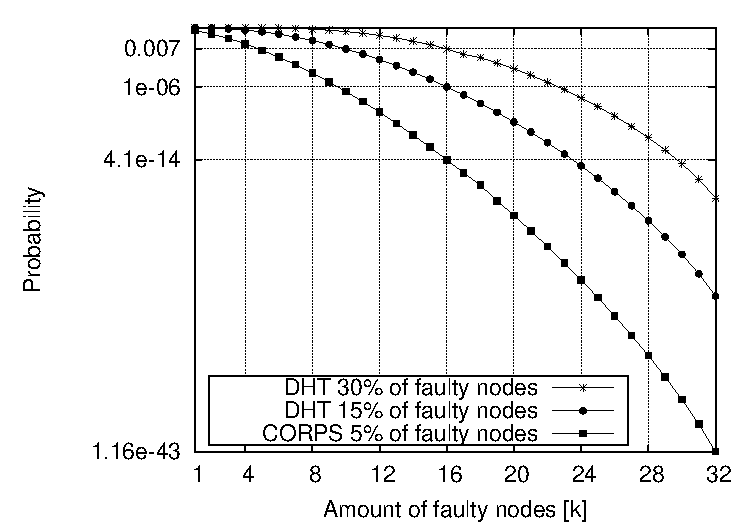
\includegraphics[scale=0.9]{perf-plot-1.pdf}
	\end{center}
	\caption{Probability of including [k] faulty/malicious nodes in the service}
	\label{graph:faulty-proportion-plot}
\end{figure}

For example, Figure~\ref{graph:faulty-proportion-plot} compares the efficiency of three different service architectures in eliminating adversarial behaviors. Every data point gives the probability that $k$ faulty/malicious nodes managed to participate in a computation that involves 32 nodes. In the absence of at least one reliable node ($k = 32$), the failure will go undetected ; but the results show that this case is extremely unlikely, regardless of the architecture. The most significant result pertains to $k = 16$: the reliable nodes detect the failure, but cannot reach a majority to recover. The graph shows that the \texttt{CORPS 5\%} architecture is much more resilient than the \texttt{DHT 30\%} architecture, by a magnitude of $10^{11}$.

% ------------------------------------------------------------------------------------------------------------------------

\section{Discussion}
1. 
% ------------------------------------------------------------------------------------------------------------------------

\section{Conclusion}


\bibliographystyle{IEEEtran}
\bibliography{references}


%------ To create Appendix with additional stuff -------%
%\newpage
%\appendix
%\section{Appendix}
%Put data files, CAD drawings, additional sketches, etc.

\end{document} 